\section{Introduction}
\label{ch:introduce}

Neutrino-nucleus coherent pion production is an inelastic interaction that produces a lepton and a pion in the forward
direction while leaving the nucleus in its initial state.  The charged current (CC) processes are
\begin{eqnarray}
\nu_{l} + \text{A} \to l^{-} + \pi^{+} + \text{A} \nonumber \\
\overline{\nu}_{l} + \text{A} \to l^{+} + \pi^{-} + \text{A}
\end{eqnarray}
and the neutral current (NC) processes are
\begin{eqnarray}
\nu_{l} + \text{A} \to \nu_{l} + \pi^{0} + \text{A} \nonumber \\
\overline{\nu}_{l} + \text{A} \to \overline{\nu}_{l} + \pi^{0} + \text{A}
\end{eqnarray}
where A is the nucleus.  For the interaction to preserve the initial state of the nucleus, the absolute value of the square of the four-momentum
exchanged with the nucleus, \tabs, must be small.
%, i.e., $\tabs\lesssim 1/R^2$, where $R$ is the radius of the nucleus.
In addition, the particle(s) exchanged with the nucleus can only carry vacuum quantum numbers in coherent scattering.  

%The square of the four-momentum exchanged with the nucleus is defined as
%\begin{equation}
%|t| = |(q-p_{\pi})^{2}| = |(p_{\nu} - p_{\mu} - p_{\pi})^{2}|,
%\end{equation}
%where $p_{\nu}$, $p_{\mu}$, and $p_{\pi}$ are the four-momentum of the neutrino, muon, and pion, respectively.  

%For neutrino (antineutrino) interactions on carbon nuclei at neutrino energy $\enu=$ 1.0 GeV, theoretical models (see
%Sec.~\ref{sec:models}) predict the rate of coherent pion production to be only $\sim$1\% ($\sim$3\%) of the total
%interaction rate for both CC and NC interactions.

Coherent pion production is not a common process; for neutrino (antineutrino) interactions on carbon nuclei at
$\enu \sim$\unit[3]{GeV}, theoretical models (see Sec.~\ref{sec:MC_bkg_Data}) predict the rate of coherent pion production
to be only $\sim$1\% ($\sim$3\%) of the total interaction rate for both CC and NC interactions.  Nonetheless, coherent
pion production is an important background for neutrino oscillation experiments, which typically operate in the range
\unit[1]{GeV}$\lesssim \enu \lesssim$ \unit[10]{GeV}.  NC coherent pion
production is an important background to $\numu\to\nue$ and $\numubar\to\nuebar$ oscillation measurements where the oscillation
signals are $\nue + N \to e^{-} + X$ and $\nuebar + N \to e^{+} + X$,
where $N$ is a target nucleon and $X$ is the hadronic final state.  NC coherent pion production yields only a \pizero\ to be
observed in the detector and if one of the two final state photons is not observed, the other can be mistaken for an electron
or positron.  CC coherent pion production is a background to measurements of \numu and \numubar disappearance at low neutrino
energy ($\enu\lesssim$ 1 GeV) where quasielastic scattering
\begin{eqnarray}
\numu + n \to \mu^{-} + p \nonumber \\
\numubar + p \to \mu^{+} + n
\end{eqnarray}
is the primary interaction process.  Coherent pion production can be mistaken for quasielastic scattering when the
$\pi^{\pm}$ is misidentified as a proton or is not detected.

This paper presents precise measurements of the \numu and \numubar CC coherent pion production cross sections on carbon
for 2 $<\enu<$ 20 GeV.  The cross sections are measured as a function of the pion energy, pion angle, and \qsq, which characterize the
coherent pion production kinematics.  A subset of these results based on this same data was published earlier~\cite{bib:minerva_coh}.
The results presented in this paper have a revised treatment of backgrounds, additional differential distributions, a new prediction of the neutrino and
antineutrino fluxes in the beam and the correlations between the neutrino and antineutrino measurements.  Also presented is a
study from the data of the possible contributions of diffractive scattering to this measurement of coherent pion production.
Accordingly, the results in this paper supersede those of Ref.~\cite{bib:minerva_coh}.

This paper is organized as follows.  Sections \ref{sec:models} and \ref{sec:before2015} describe two existing models and the experimental
state of the field prior to this work.  Section \ref{sec:diffractiveIntro} introduces diffractive scattering of neutrinos off hydrogen,
an important and closely related process that is studied here.  Sections \ref{sec:NuMI_N_me}-\ref{sec:event_selection} describe the experiment,
the event selection and the reconstruction of candidate events.  Sections \ref{sec:bg_tuning}-\ref{sec:systematics} explain the measurement
of the cross sections and their systematic uncertainties.  Sections \ref{sec:measured_cross_sections}-\ref{sec:conclusions} present the
results and their interpretation.


\section{Models}
\label{sec:models}

PCAC coherent
models~\cite{bib:coh_pcac3,bib:coh_pcac4,bib:coh_pcac5,bib:coh_pcac6,bib:coh_pcac7,bib:coh_pcac10}
and \cite{bib:RS,bib:RS2,bib:berger_sehgal, bib:kartavtsev, bib:manny}
are a class of coherent pion production models that are based on
Adler's PCAC theorem~\cite{bib:adler_pcac} (Partial Conservation of Axial Current, or in modern language,
spontaneous breaking of chiral symmetry in QCD) which can be used to relate coherent pion production
at $Q^2=-(p_{\nu}-p_{l})^{2}=0$ to elastic pion-nucleus scattering.  Here, $p_{\nu}$ ($p_{l}$) is the
four-momentum of the incoming neutrino (outgoing charged lepton).  In this picture of coherent pion production,
the intermediate weak boson fluctuates to a virtual pion, which scatters elastically off the nucleus, as shown in
the Pomeron (\Pom) diagram of Fig.~\ref{fig:feyman_pcac_coh_cc_nc}.

\subsection{Rein-Sehgal Model}
\label{sec:Rein-Sehgal}

\begin{figure}[tp]
\centering
\mbox{
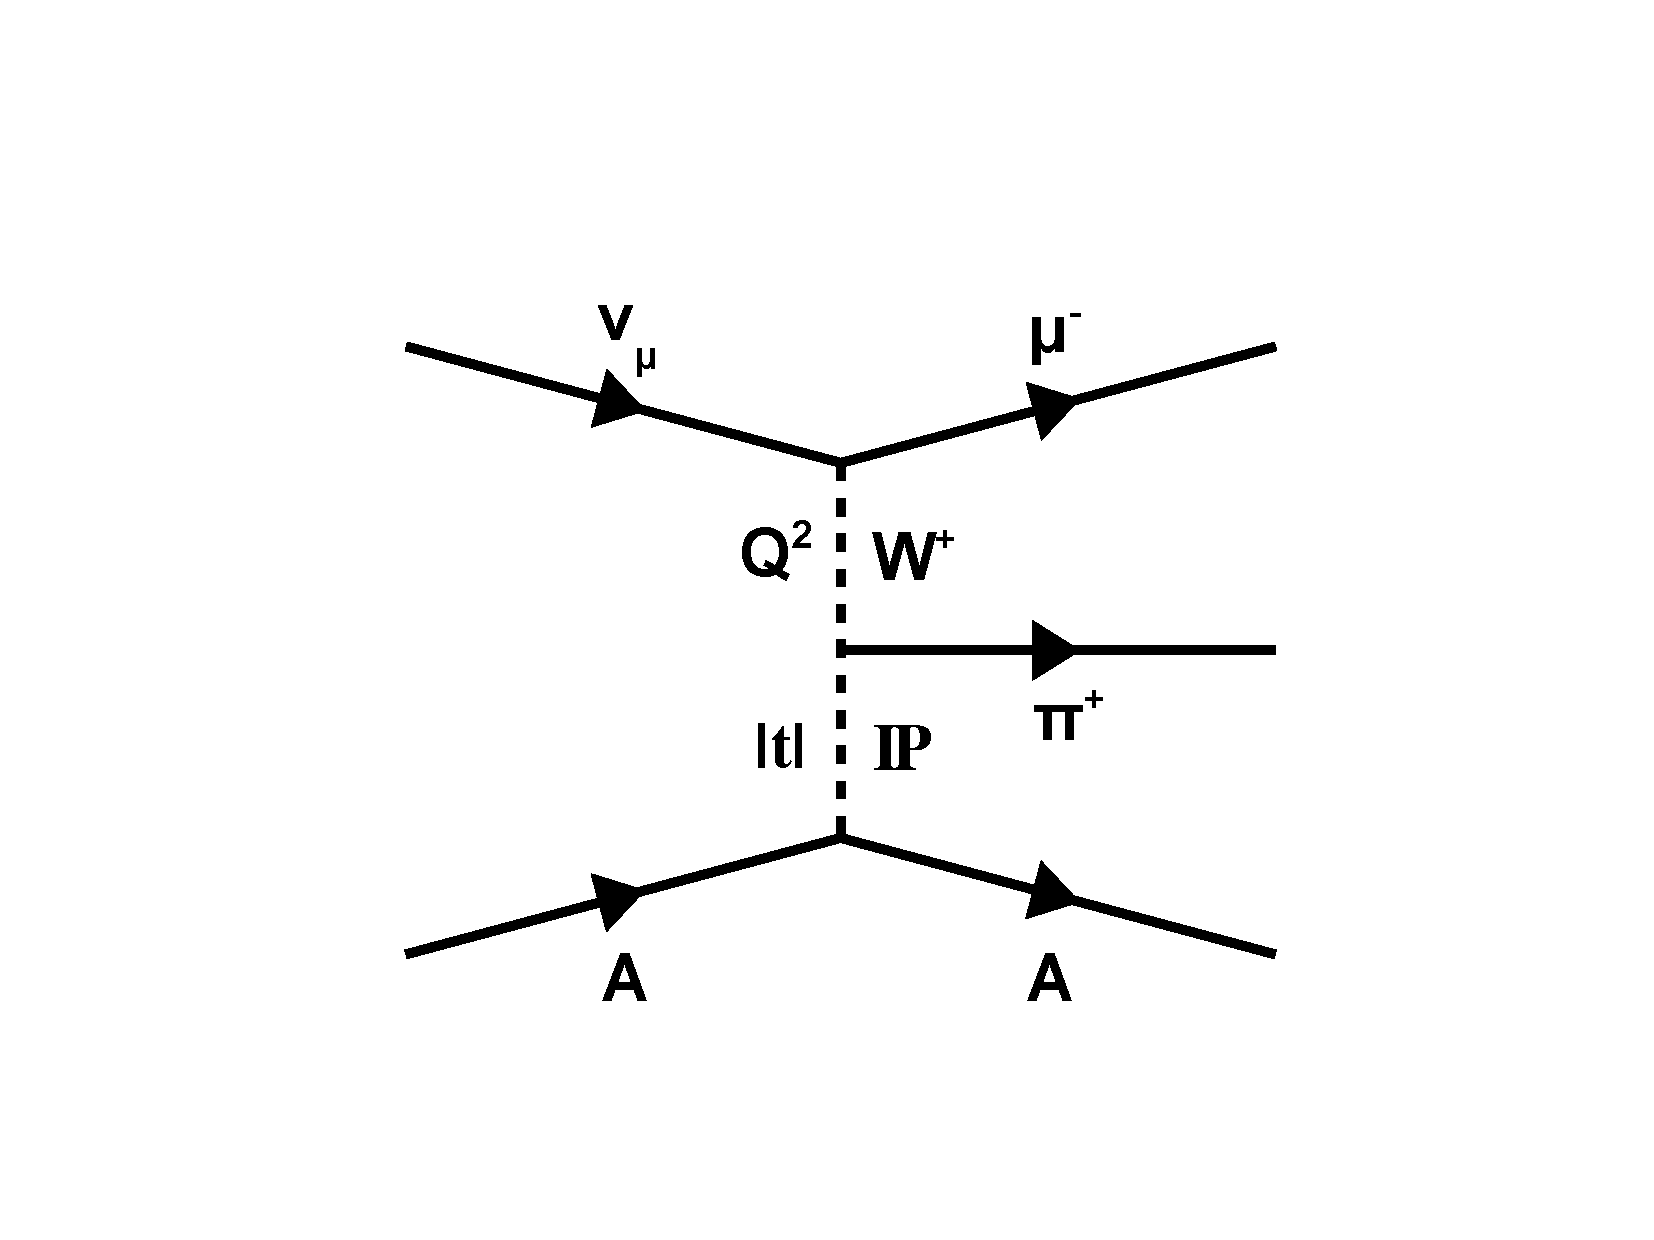
\includegraphics[width=0.49\columnwidth]{figures/FeynmanDiagrams/coh_cc.pdf}
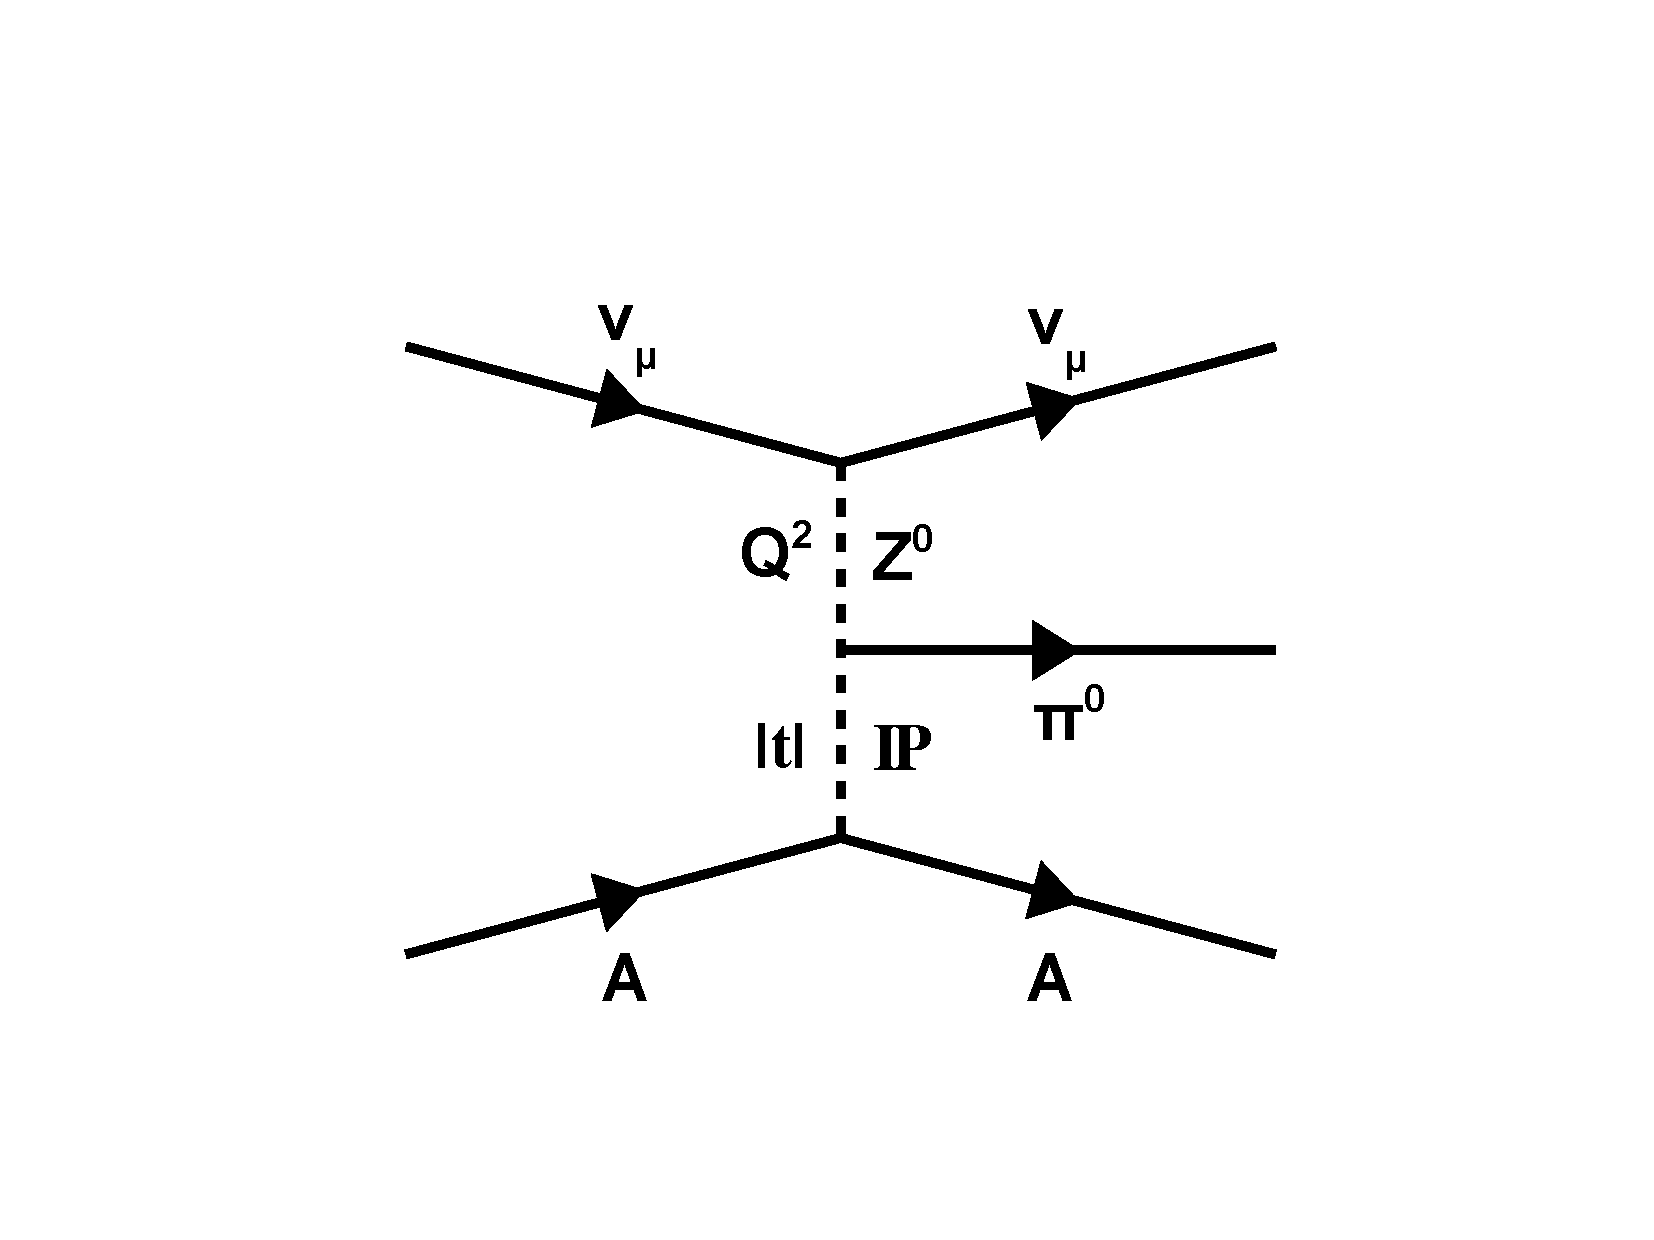
\includegraphics[width=0.49\columnwidth]{figures/FeynmanDiagrams/coh_nc.pdf}}
\caption[CC and NC neutrino-nucleus coherent pion production in the PCAC picture]{CC (left) and NC (right) neutrino-nucleus
																				  coherent pion production in the PCAC picture.}
\label{fig:feyman_pcac_coh_cc_nc}
\end{figure}

The Rein-Sehgal coherent model~\cite{bib:RS,bib:RS2} is the most widely used PCAC coherent pion production model in
neutrino event generators.  The Rein-Sehgal model extrapolates the Adler coherent cross section result to $\qsq > 0$
using a multiplicative axial-vector dipole form factor
\begin{equation}
F_{A} = \frac{M_{A}^{2}}{Q^{2} + M_{A}^{2}},
\end{equation}
where $M_{A} \approx$ 1 GeV is the axial vector mass.  The Rein-Sehgal model assumes no vector current contribution in
this extrapolation, and therefore predicts equal cross sections for neutrinos and antineutrinos.

The Rein-Sehgal model calculates the $\pi^{\pm}$A elastic cross section using charged pion-nucleon ($\pi^{\pm}N$)
scattering data.

The differential CC coherent pion production cross section calculated by the Rein-Sehgal model is
\begin{eqnarray}
\label{eq:rs_cccoh_xsec}
\frac{d\sigma_{coh}^{CC}}{d\qsq dyd\tabs} &= \frac{G^{2}f_{\pi^{\pm}}^{2}}{2\pi}\frac{(1-y)}{y}\frac{M_{A}^{2}}{Q^{2} + M_{A}^{2}}A^{2} \nonumber \\
&\times \exp\left(-\frac{1}{3}R_{0}^{2}A^{2/3}\tabs-\frac{9A^{1/3}}{16\pi R_{0}^{2}}\sigma_{inel}^{\pi^{\pm}N}(\epi)\right)\nonumber\\
&\times \frac{1}{16\pi}\left(\sigma_{tot}^{\pi^{\pm}N}(\epi)\right)^{2}(1+r^{2}),
%\right]_{E_{\pi}=yE_{\nu}}.
%\frac{d\sigma_{coh}^{CC}}{d\qsq dyd\tabs} &= \frac{G^{2}f_{\pi^{\pm}}^{2}}{2\pi}\frac{(1-y)}{y}\frac{M_{A}^{2}}{Q^{2} + M_{A}^{2}} \nonumber \\
%&\times \left[A^{2}\exp\left(-\frac{1}{3}R_{0}^{2}A^{2/3}\tabs\right)\exp\left(-\frac{9A^{1/3}}{16\pi R_{0}^{2}}\sigma_{inel}^{\pi^{\pm}\text{N}}\right)\frac{1}{16\pi}\Big[\sigma_{tot}^{\pi^{\pm}\text{N}}\Big]^{2}(1+r^{2})\right]_{E_{\pi}=yE_{\nu}}. %\nonumber \\
%&\times \left[\left(1-\frac{1}{2}\frac{Q^{2}_{min}}{Q^{2}+m^{2}_{\pi}}\right)^{2}+\frac{y}{4}\frac{Q^{2}_{min}(Q^{2}-Q^{2}_{min})}{(Q^{2}+m^{2}_{\pi})^{2}}\right] \nonumber \\
%&\times \theta(\qsq - \qsq_{min})\theta(y - y_{min})\theta(y_{max} - y)
\end{eqnarray}
where the pion energy $\epi=y\enu$, $A$ is the atomic number of the target nucleus, $f_\pi$ is the pion decay constant,
$R_0$ is the nuclear length scale $\sim 1$~fm and $r = \text{Re}f(0)/\text{Im}f(0)$ is the ratio of the real and imaginary
parts of the $\pi^{\pm}N$ forward scattering amplitude.  The exponential dependence in \tabs is the consequence of a simple
gaussian model for the nuclear form factor in $\pi A$ elastic scattering. The Rein-Sehgal model calculates the NC
differential cross section from Eq.~(\ref{eq:rs_cccoh_xsec}) using $f_{\pi^{0}} = f_{\pi^{\pm}}/\sqrt{2}$ and assuming that
the $\pi^{\pm}N$ and $\pi^{0}N$ cross sections are equal.

The Rein-Sehgal model corrects the CC differential cross section (Eq.~\ref{eq:rs_cccoh_xsec}) for the mass of the final state
lepton \cite{bib:RS2,bib:lepton_mass_corr}.  The correction, proposed by Adler \cite{bib:lepton_mass_corr}, is
\begin{eqnarray}
C &= \left(1-\frac{1}{2}\frac{Q^{2}_{min}}{Q^{2}+m^{2}_{\pi}}\right)^{2}+\frac{y}{4}\frac{Q^{2}_{min}(Q^{2}-Q^{2}_{min})}{(Q^{2}+m^{2}_{\pi})^{2}} \\
&\times \theta(\qsq - \qsq_{min})\theta(y - y_{min})\theta(y_{max} - y), \nonumber
\end{eqnarray}
where $Q^{2}_{min} = m^{2}_{l}y/(1-y)$ is the kinematic minimum \qsq, $y_{min} = m_{\pi}/\enu$ and $y_{max} = 1 - m_{l}/\enu$ are the kinematic minimum and maximum $y$, and $m_{l}$ and $m_{\pi}$ are the final state lepton and pion masses.

The Rein-Sehgal model predicts that both $\sigma_{coh}^{CC}(\enu)$ and $\sigma_{coh}^{NC}(\enu)$
scale with $A$ approximately as $A^{1/3}$, as a result of the nuclear coherence condition and pion absorption effects.
%, and \tabs-dependence.   Leo asks: oh?



\subsection{Berger-Sehgal Model}
\label{sec::Berger-Sehgal}

The cross section of Eq.~(\ref{eq:rs_cccoh_xsec}) is differential in three variables but coherent scattering only occurs in
a limited region of the phase space.  Newer models~\cite{bib:berger_sehgal, bib:kartavtsev, bib:manny} use data from pion-nucleus
elastic scattering.  These show that coherent scattering predominantly occurs at \qsq$\sim\mathcal{O}(m_\pi^2), ~\nu^2 = (E_\nu - E_l)^2 \gg \qsq$
and $\tabs\lesssim 1/R^2$, where $E_\nu$ ($E_l$) is the energy of the incoming neutrino (outgoing lepton) and $R$ is the radius of the nucleus.
In particular, coherent scattering creates a sharp increase in the slope of $d\sigma/d\tabs$ as \tabs approaches
\tmin$\sim \frac{ (Q^2+m_\pi^2)^2}{2\nu}$, the minimum kinematically possible \tabs.
The Berger-Sehgal PCAC coherent model \cite{bib:berger_sehgal} is a modification of the Rein-Sehgal model where the
parameterization of the $\pi^{\pm}$A elastic scattering cross section is instead fit to charged pion-carbon ($\pi^{\pm}$C)
elastic scattering data and scaled to other nuclei.  This approach avoids some of the uncertainties from modeling nuclear effects,
\textit{e.g.} pion absorption, in the Rein-Sehgal parameterization.  In the Berger-Sehgal model, coherent cross sections scale
as $A^{2/3}$.
%The Berger-Sehgal model parameterizes the differential$\pi^{\pm}$C elastic cross section as
%\begin{equation}
%\frac{d\sigma_{el}^{\pi^{\pm}\text{C}}}{d\tabs} = A_{1}e^{-b_{1}\tabs},
%\label{eq:bs_piC_xsec}
%\end{equation}
%where the normalization $A_{1}$ and slope $b_{1}$ are functions of \epi and are fit to data (Figure~\ref{fig:rs_bs_pion_carbon_elastic_xsec}).
The comparison of Rein-Sehgal and Berger-Sehgal calculations of $\sigma_{el}^{\pi^{\pm}\text{C}}$ in
Fig.~\ref{fig:rs_bs_pion_carbon_elastic_xsec} shows that while the two calculations agree for $|\vec{p}_{\pi}|\gtrsim0.7$ GeV,
the Rein-Sehgal predicts a much larger cross section in the $\Delta$ resonance dominated region, $|\vec{p}_{\pi}|\sim0.3$ GeV.
\begin{figure}[tpb]
\centering
%\includegraphics[width=1.0\columnwidth]{figures/CoherentChapter/rs_bs_pion_carbon_elastic_xsec.pdf}
%\caption[Rein-Sehgal and Berger-Sehgal pion-carbon elastic scattering cross sections]{The plot on the left is the Rein-Sehgal (dashed line) and Berger-Sehgal (solid line) predictions of the pion-carbon elastic scattering cross section as a function of the pion momentum in the laboratory frame.  The table on the right are the parameters for the Berger-Sehgal pion-carbon elastic scattering cross section determined from fitting pion-carbon-elastic scattering data.  The plot and table are from \cite{bib:berger_sehgal}}
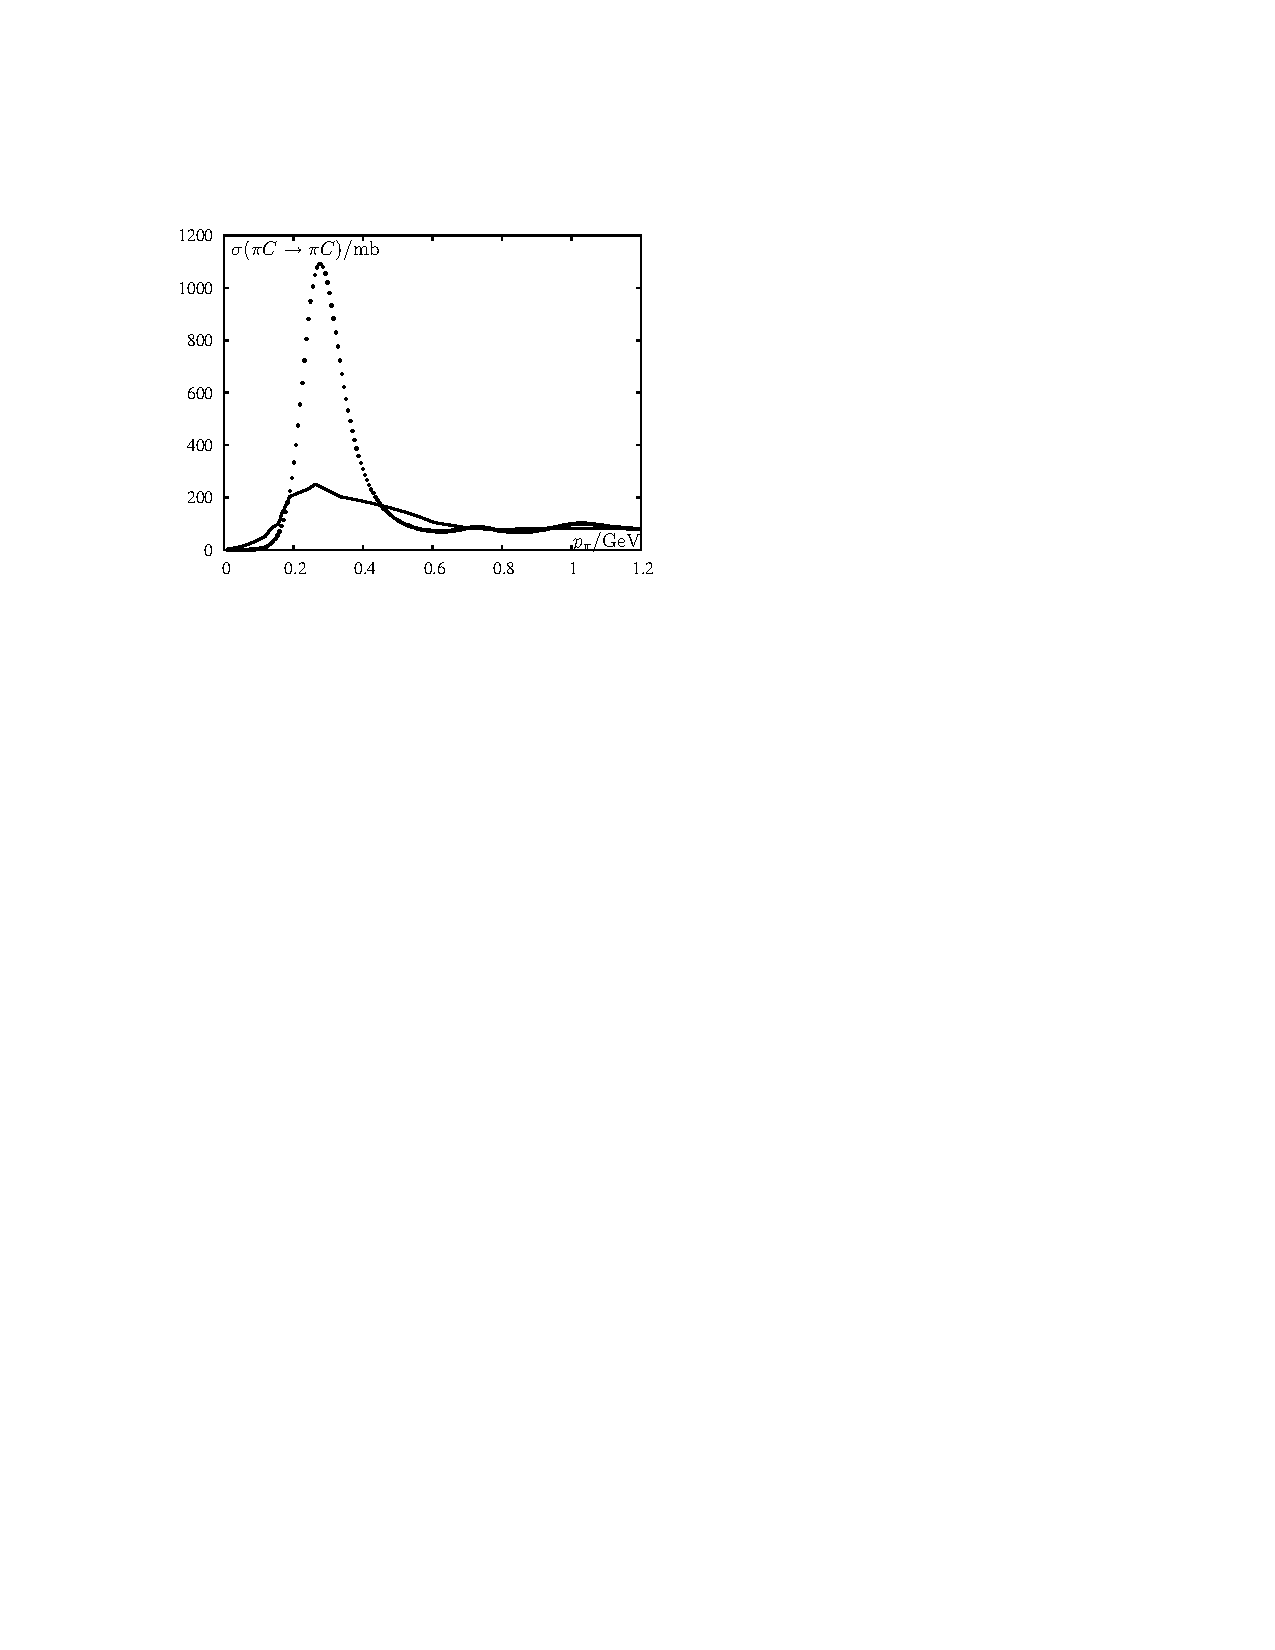
\includegraphics[width=1.0\columnwidth]{figures/CoherentChapter/rs_bs_pion_carbon_elastic_xsec_left.pdf}
\caption[Rein-Sehgal and Berger-Sehgal pion-carbon elastic scattering cross sections]{The Rein-Sehgal (dashed line)
		 and Berger-Sehgal (solid line) pion-carbon elastic scattering cross sections as a function of the pion momentum
		 in the laboratory frame.  From \cite{bib:berger_sehgal}.}
\label{fig:rs_bs_pion_carbon_elastic_xsec}
\end{figure}

\section{Earlier Measurements}
\label{sec:before2015}

Coherent CC interactions can be identified by requiring that the observed final state consist only of a charged lepton and
pion (the target nucleus is not observed since the energy transferred to the nucleus is small) and small \tabs.  From 
the assumption of zero energy transfer to the nucleus,
\begin{eqnarray}
\tabs &= |( p_{\nu_{l}} - p_{l} - p_{\pi})^{2}| \nonumber \\
& \approx \left(\displaystyle \sum_{i=\mu,\pi} E_i-p_{i,L}\right)^2+\left| \displaystyle \sum_{i=\mu,\pi}\vec{p}_{i,T}\right| ^2,
\label{eq:t_calc} 
\end{eqnarray}
where $p_{\nu_{l}}$, $p_{l}$, and $p_{\pi}$ are the four-momenta of the neutrino, charged lepton, and pion, respectively,
and $\vec{p}_{T}$ and $p_{L}$ are transverse and longitudinal momenta with respect to the incoming neutrino direction.
The neutrino four-momentum is determined by assuming that its direction is that of the neutrino beam and its energy is
$\enu = E_{l} + \epi$.
%where the energy transferred to the nucleus is ignored since it will be small at low \tabs.

For NC coherent interactions, the final state neutrino is not observed and the observed final state is a lone $\pi^{0}$.
Neither \enu nor \tabs can be measured.
Since \tabs is not available, experiments isolate NC coherent interactions using the condition
\begin{equation}
\epi(1-\cos\thetapi) < \frac{1}{R}, 
\end{equation}
where \thetapi is the angle between the pion and incoming neutrino directions.  This condition follows from the
$\tabs \lesssim 1/R^2$ condition for coherent scattering at \mbox{$\qsq\approx$ 0 \cite{bib:lackner}}.  However, imposing
selection requirements on the pion kinematics creates implicit selection requirements on the lepton kinematics and
\qsq (see Eq.~\ref{eq:t_calc}).
Consequently, NC coherent pion production measurements must make model-dependent assumptions about the \qsq dependence of the
coherent scattering cross section when correcting for the inefficiency of this selection requirement.  

Since \enu cannot be measured, NC coherent pion production measurements are averaged over the energy spectrum of a neutrino
beam.  These experimental limitations of NC coherent pion production measurements increase the importance of CC coherent
pion production measurements, which in the PCAC picture provide a constraint on the NC reaction.

Many measurements of 
NC~\cite{bib:coh_nc_AP,bib:coh_nc_garg,bib:coh_nc_charm,bib:coh_nc_cc_skat,bib:coh_nc_fnal,bib:coh_nc_nomad,bib:coh_nc_sb,bib:coh_nc_mb,bib:coh_nc_minos}
and
CC~\cite{bib:coh_nc_cc_skat,bib:coh_cc_bebc1,bib:coh_cc_fnal1,bib:coh_cc_bebc2,bib:coh_cc_fnal2,bib:coh_cc_fnal3,bib:coh_cc_charm,
bib:coh_cc_k2k,bib:coh_cc_sb,bib:coh_cc_argo}
%MOVE THESE TO LATER SINCE THIS IS A LIST OF "BEFORE 2015" - well, it was.  But now it isn't
coherent pion production have been made at neutrino energies of 1 $\lesssim\enu\lesssim$ 100 GeV using both \numu and \numubar
beams and a variety of scattering target materials (carbon, neon, aluminum, argon, Freon, glass, marble and iron).  Measurements
made before the discovery of neutrino oscillations were mostly made at $\enu>$ 10 GeV.
Precise measurements at 1 $\lesssim\enu\lesssim$ 10 GeV are now needed for constraining backgrounds in
oscillation measurements in high intensity \numu and \numubar beams.
% that operate at 1 $\lesssim\enu\lesssim$ 10 GeV.

Early measurements of the NC coherent pion production cross section as a function of
\enu~\cite{bib:coh_nc_AP,bib:coh_nc_garg,bib:coh_nc_charm} are shown in Fig.~\ref{fig:charm_coh_nc}.  They were made
using different scattering target materials and, for the purpose of comparison, are scaled in Fig.~\ref{fig:charm_coh_nc}
to a marble scattering target with an effective $A$ = 20 using the $A^{1/3}$ dependence of the cross section.
While the Rein-Sehgal model prediction agrees with the measured cross sections within their uncertainties, the uncertainties
are large ($\gtrsim$ 30\% \cite{bib:coh_nc_nomad}).

\begin{figure}[tpb]
\centering
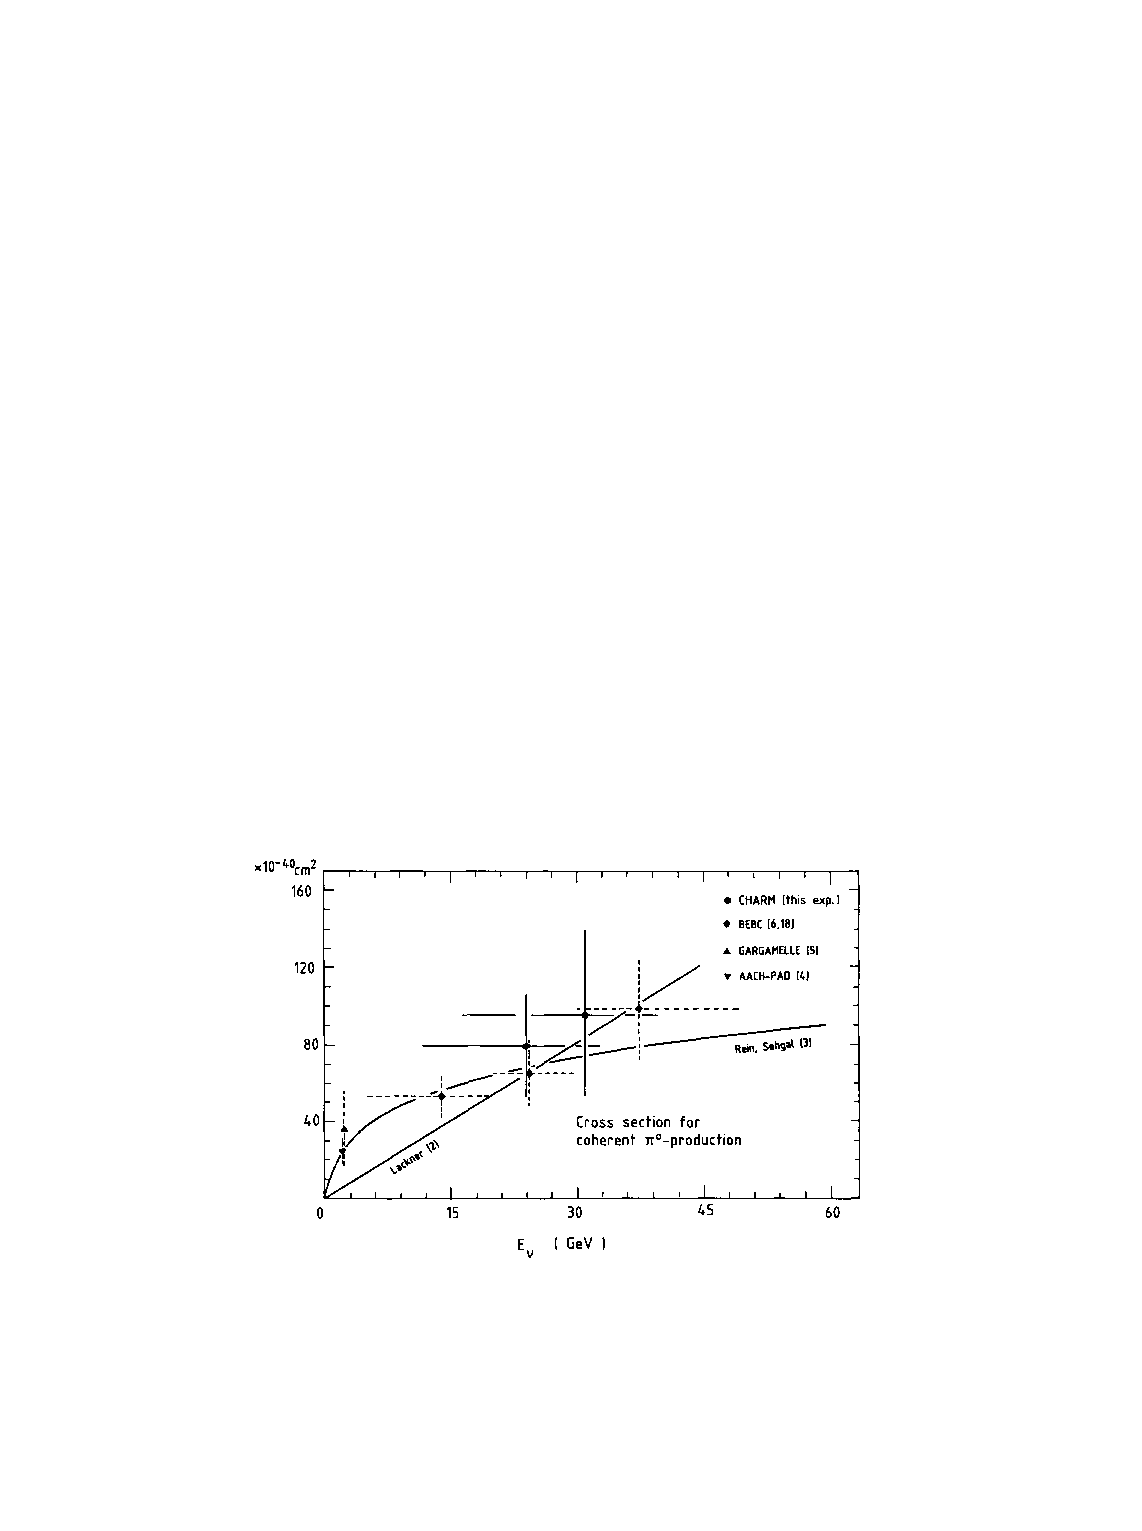
\includegraphics[width=0.8\columnwidth]{figures/CoherentChapter/charm_coh_nc.pdf}
\caption[Early measurements of NC coherent pion production]
	{Early measurements of the NC coherent pion production cross section.  The horizontal error bars represent the range
	of neutrino energies sampled by the measurement.  The figure is from \cite{bib:coh_nc_charm}.}
\label{fig:charm_coh_nc}
\end{figure}

Early measurements of the \numu and \numubar CC coherent pion production cross sections as a function of
\enu~\cite{bib:coh_nc_cc_skat,bib:coh_cc_bebc1,bib:coh_cc_fnal1,bib:coh_cc_bebc2,bib:coh_cc_fnal2,bib:coh_cc_fnal3,bib:coh_cc_charm},
along with the early measurements of the NC coherent pion production cross
section~\cite{bib:coh_nc_AP,bib:coh_nc_garg,bib:coh_nc_charm,bib:coh_nc_cc_skat}, are shown in Fig.~\ref{fig:charm_coh_cc}.
For comparison, the measurements in Fig.~\ref{fig:charm_coh_cc} are scaled to a glass scattering target with an effective
$A$ = 20.1, and the NC measurements are additionally scaled by a factor of 2 per the relation between the CC and NC coherent
cross sections from Adler's PCAC theorem.  These early CC measurements isolated CC coherent interactions by requiring a
forward $\mu^{\mp}$ and $\pi^{\pm}$, the absence of additional particles emerging from the interaction vertex, and small \tabs.
The Rein-Sehgal model agrees well with most of the measurements, which supports the predicted $A^{1/3}$ dependence and the
2-to-1 relationship between the CC and NC coherent cross sections.
\begin{figure}[tpb]
\centering
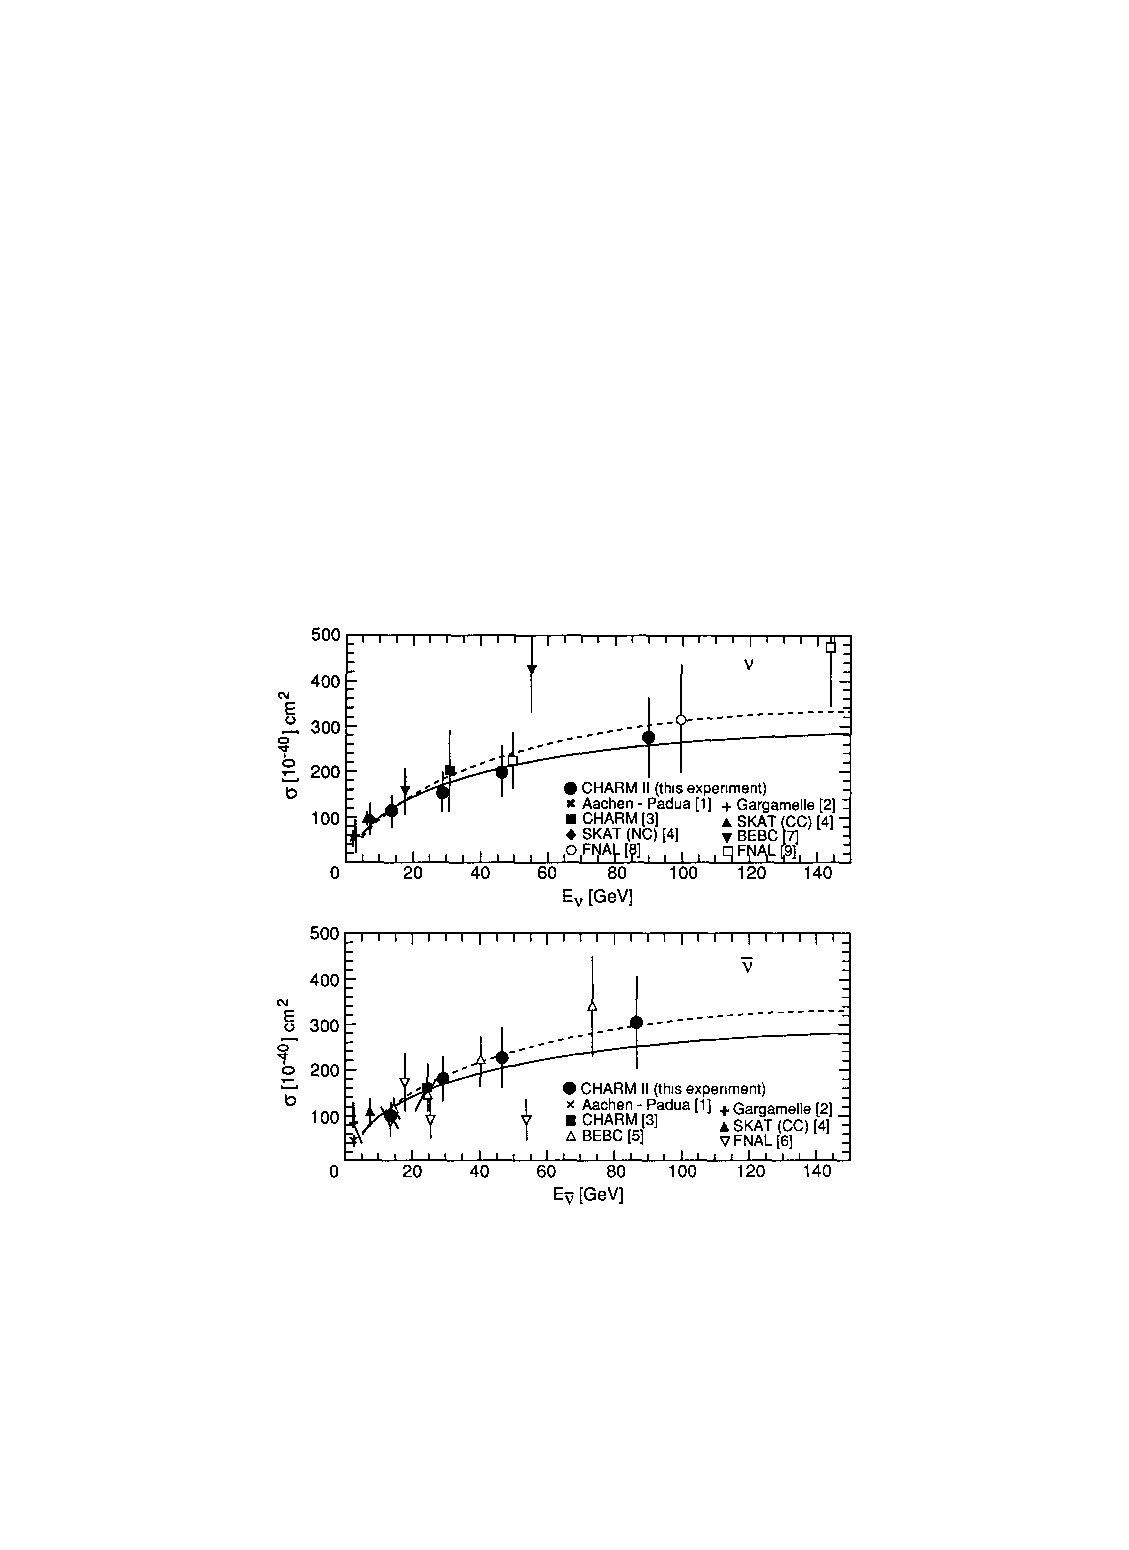
\includegraphics[width=0.8\columnwidth]{figures/CoherentChapter/charm_coh_cc.pdf}
\caption[Early measurements of CC coherent pion production]{Early measurements of the \numu (top) and \numubar (bottom) CC
	coherent pion production cross sections.  The solid line is the Rein-Sehgal model prediction.  The figure is
	from~\cite{bib:coh_cc_charm}.}
\label{fig:charm_coh_cc}
\end{figure}

The only measurements of NC coherent pion production at $\enu<$ 2 GeV were made recently by the MiniBooNE~\cite{bib:coh_nc_mb}
and SciBooNE \cite{bib:coh_nc_sb} experiments.  The MiniBooNE measurement was made using a mineral oil target (CH$_{2}$) at a
peak \enu of 0.7 GeV.  MiniBooNE measured the NC coherent pion production cross section to be $(19.5\pm2.7)$\% of the
total (coherent + non-coherent) NC single $\pi^{0}$ production cross section.  The SciBooNE measurement was made using a
polystyrene target (CH) at an average \enu  of 0.8 GeV.  SciBooNE measured the ratio of the NC coherent pion
production cross section to the \numu CC total (all scattering processes) cross section to be $(1.16\pm0.24)\times10^{-2}$.  
%These measurements provide strong evidence for NC coherent pion production at $\enu<$ 2 GeV.

The first searches for \numu CC coherent pion production at $\enu\lesssim$ 2 GeV were  performed  by the K2K~\cite{bib:coh_cc_k2k}
and SciBooNE~\cite{bib:coh_cc_sb} experiments.  These experiments used the same CH-based detector in two different neutrino beams.  
Neither could measure \tabs since the detector did not provide adequate containment of the pion to allow accurate measurement of
the pion energy, and instead searched for coherent scattering at low \qsq.
Neither experiment found evidence for CC coherent interactions after subtracting the predicted non-coherent background
(Figs.~\ref{fig:k2k_coh_cc} and~\ref{fig:sb_coh_cc}).  The experiments reported upper limits on the ratio of the \numu CC
coherent pion production cross section to the \numu CC total cross section, which are listed in Table~\ref{tab:k2k_sb_coh_cc}.

The non-observation of \numu CC coherent pion production at $\enu<$ 2 GeV is in contradiction to the the Rein-Sehgal coherent model.
It should be noted that a search for coherent pion production in \qsq is model dependent.  In addition, both the K2K and
SciBooNE measurements constrained their background prediction using interactions with activity near the interaction vertex in
addition to that from the muon and pion.  The background prediction is therefore sensitive to the modeling of nuclear effects
which are poorly understood (see Sec.~\ref{sec:bg_tuning}).

\begin{figure}[tpb]
\centering
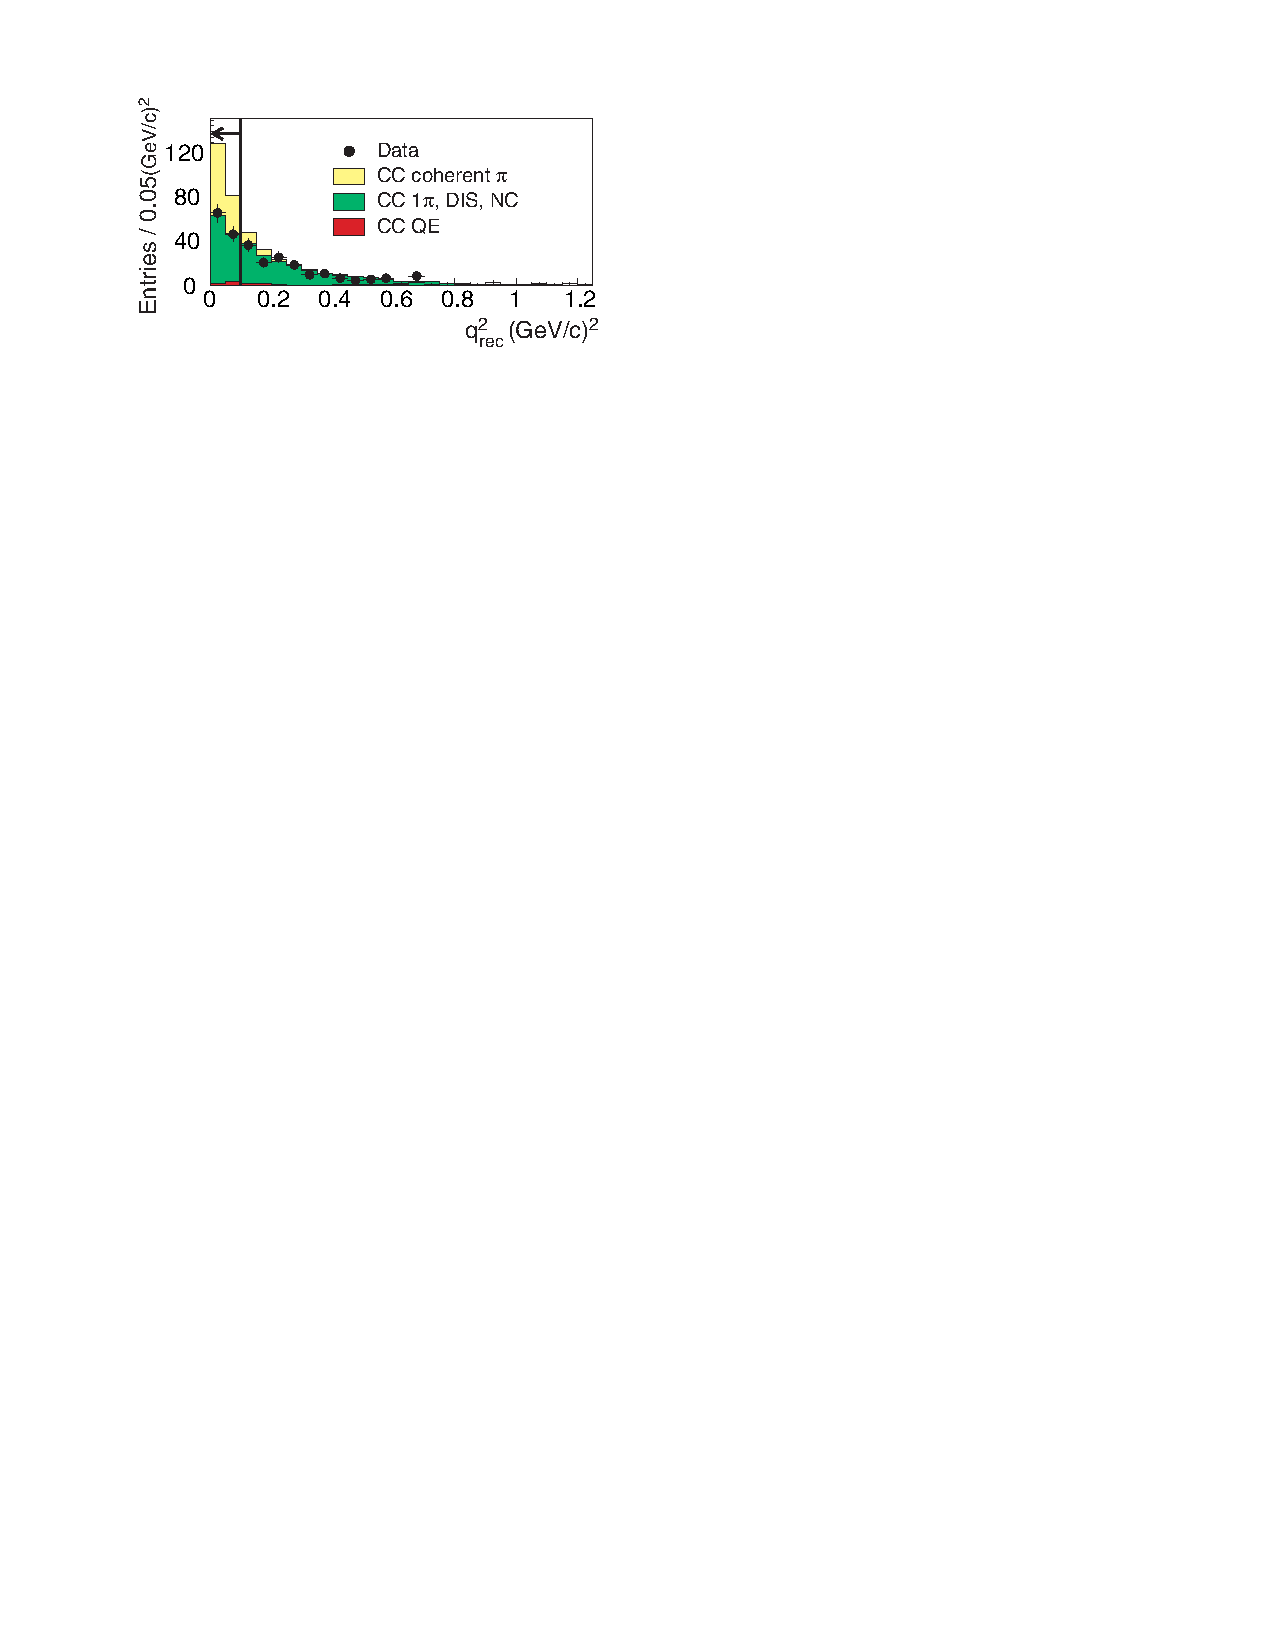
\includegraphics[width=0.8\columnwidth]{figures/CoherentChapter/k2k_coh_cc.pdf}
\caption[Search for \numu CC coherent pion production at K2K]
	{The data and simulated \qsq distributions for \numu CC coherent pion production candidates at K2K.  The figure is
	from~\cite{bib:coh_cc_k2k}.}
\label{fig:k2k_coh_cc}
\end{figure}

\begin{figure}[tpb]
\centering
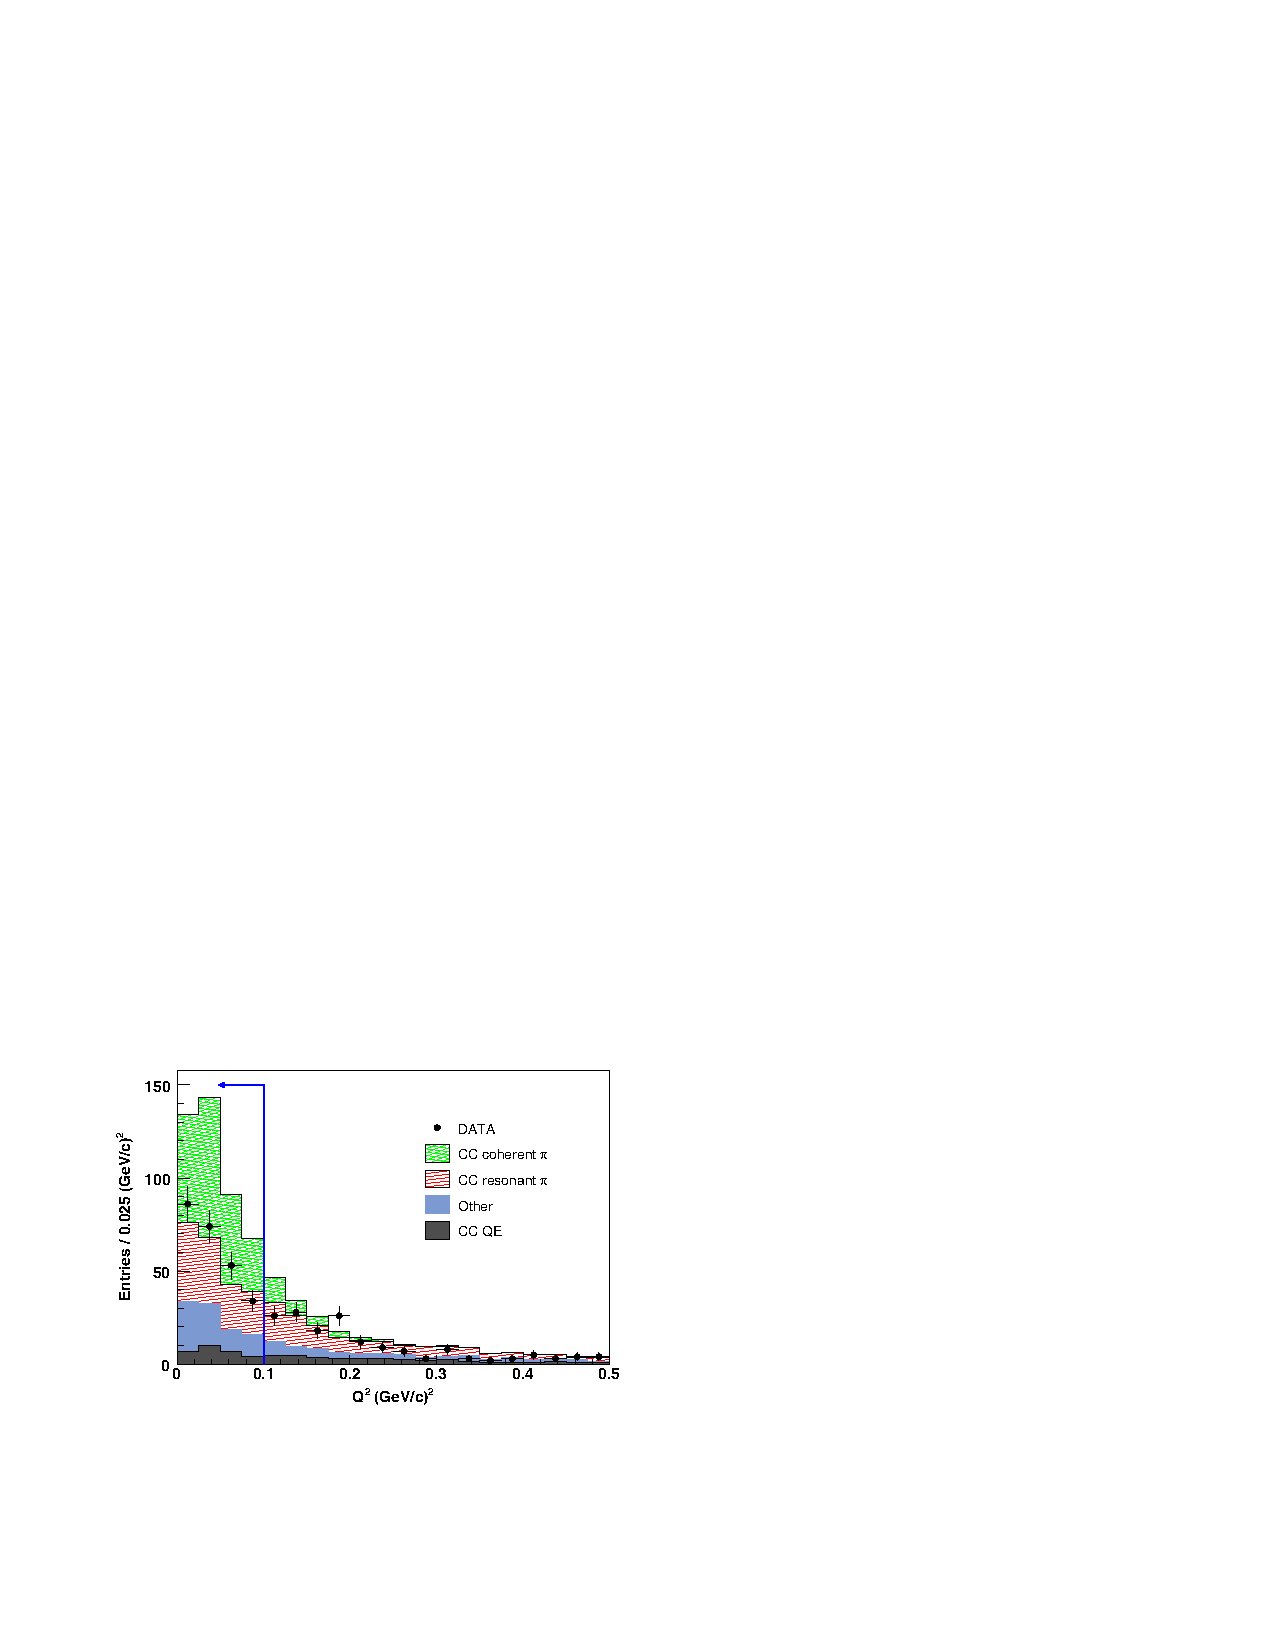
\includegraphics[width=0.8\columnwidth]{figures/CoherentChapter/sb_coh_cc.pdf}
\caption[Search for \numu CC coherent pion production at SciBooNE]{The data and simulated \qsq distributions for \numu CC
	coherent pion production candidates at SciBooNE.  The figure is from~\cite{bib:coh_cc_sb}.}
\label{fig:sb_coh_cc}
\end{figure}

\begin{table}[h!]
%\small
\begin{center}
\begin{tabular}{ c | c | c }
%\hline
%Name & Symbol & Charge & Mass  \\
Experiment & $\sigma_{CC}^{coh} / \sigma_{CC}^{tot}$ (90\% C.L.) & $\langle\enu\rangle$ (GeV) \\
\hline
K2K & $<$ 0.6 $\times$ 10$^{-2}$ & 1.3 \\
SciBooNE & $<$ 0.67 $\times$ 10$^{-2}$ & 1.1 \\
SciBooNE & $<$ 1.36 $\times$ 10$^{-2}$ & 2.2 \\
\end{tabular}
\end{center}
\caption[Upper limits on the \numu CC coherent pion production cross section reported by K2K and SciBooNE]
	{The upper limits on the ratio of the \numu CC coherent pion production cross section to the \numu CC total cross
	section, $\sigma_{CC}^{coh} / \sigma_{CC}^{tot}$, reported by K2K~\cite{bib:coh_cc_k2k} and SciBooNE~\cite{bib:coh_cc_sb}.}
\label{tab:k2k_sb_coh_cc}
\end{table}

The non-observation of CC coherent pion production at $\enu\lesssim$ 2 GeV posed a problem for both theorists and neutrino
oscillation experiments; production models are unable to reconcile it with the observation of the NC reaction at the same \enu.
To account for the theoretical and experimental disagreement, the T2K neutrino oscillation measurement, which operates at
\enu $\approx\xspace$ 0.6 GeV, applied a 100\% uncertainty on their predicted CC coherent interaction
rate, while applying a 30\% uncertainty on their predicted NC coherent interaction rate \cite{bib:t2k_osc}.  
%Neutrino-nucleus interactions are the largest source of systematic uncertainty in the T2K $\numu\to\nue$ oscillation and $\numu$ disappearance measurements (Figure~\ref{fig:t2k_osc_unc}), and the predicted rate of coherent interactions is a significant contribution to the uncertainty \cite{bib:t2k_osc}.

%\begin{figure}[!htpb]
%\centering
%\includegraphics[width=0.7\columnwidth]{figures/CoherentChapter/t2k_osc_unc.pdf}
%\caption[T2K systematic uncertainties]{The systematic uncertainties on the predictions of \numu CC and \nue CC interactions in the Super Kamiokande (SK) far detector of the T2K neutrino oscillation experiment.  Constraints on the neutrino beam flux and neutrino interaction predictions are obtained from the ND280 near detector.  The table is from \cite{bib:t2k_osc}.}
%\label{fig:t2k_osc_unc}
%\end{figure}

Precise measurements of neutrino-nucleus coherent pion production at 1 $\lesssim\enu\lesssim$ 10 GeV are needed for
testing coherent pion production models and reducing systematic uncertainties in neutrino oscillation measurements.  



\section{Diffractive Scattering}
\label{sec:diffractiveIntro}

Diffractive pion production, $\nu_\mu p\to \mu^-\pi^+ p$ (Fig.~\ref{fig:diffractive_diagram})
is a process similar to coherent scattering but for single proton.  It produces a muon and charged pion in the forward direction
while leaving the nucleus, {\it i.e.} the proton, intact and with minimal recoil.  
Like coherent scattering, diffractive production occurs at low \tabs.  Unlike coherent scattering, the recoil
proton does absorb some kinetic energy, making it potentially visible in the detector.  There are also resonant and non-resonant
processes that occur in a broader range of \tabs.  At low \tabs these may interfere with the diffractive process
which complicates the prediction of the process.

Diffractive scattering is experimentally indistinguishable from coherent scattering when the recoil proton is
below detection threshold.  A \numu / \numubar CC sample in the \minerva tracker may contain diffractive
scattering interactions since the CH scintillator contains free
protons.  Diffractive scattering was not included in the simulated backgrounds to the coherent process, so
the measured coherent cross section may therefore contain a contribution from it.  It is not coherent scattering on carbon
and is therefore a potential background to this measurement.  One of the new results presented here is that in fact this
potential background has a rate consistent with zero.

\begin{figure}[tpb]
\begin{center}
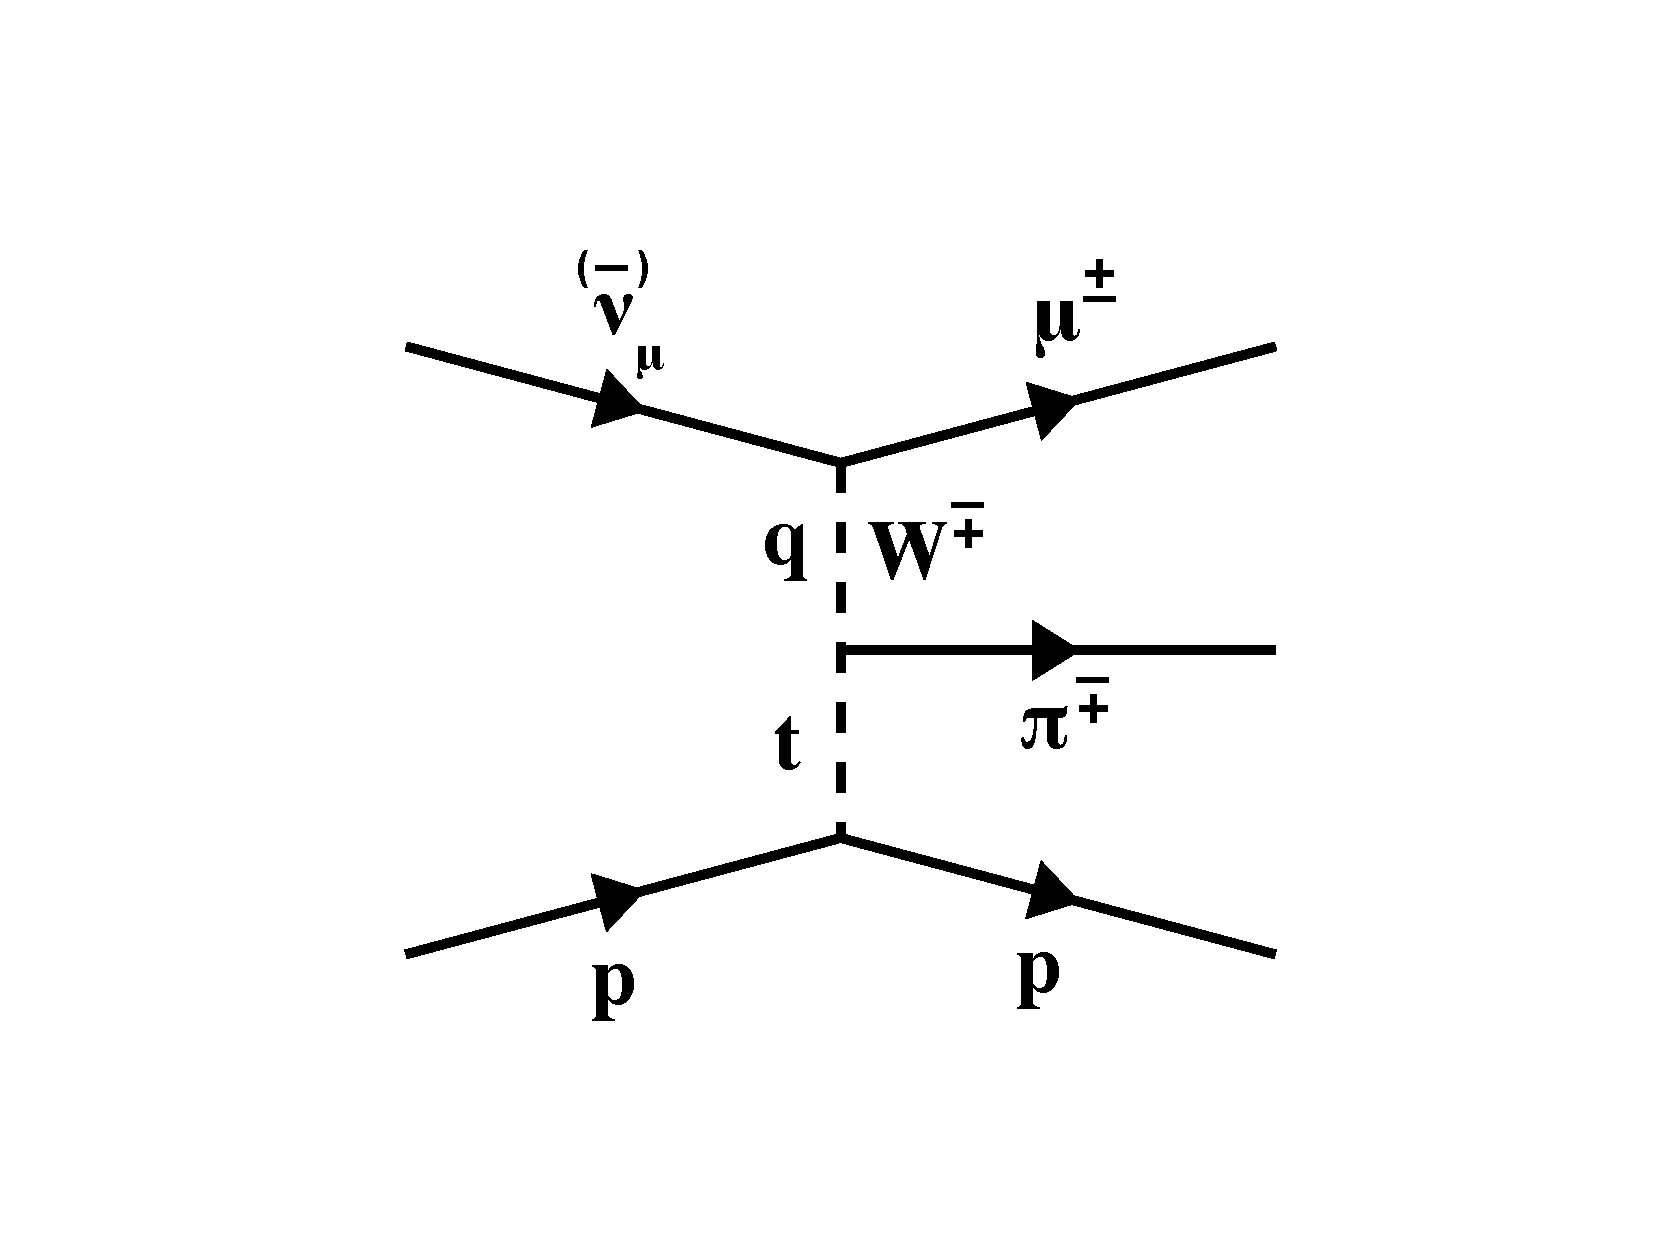
\includegraphics[width=0.8\columnwidth]{figures/Diffractive/DiffractiveDiagram.pdf}
\caption[Diffractive scattering in the PCAC picture]{Diffractive pion production on a free proton.}
\label{fig:diffractive_diagram}
\end{center}
\end{figure}

An important difference between coherent and diffractive scattering is the \tabs-dependence of the cross sections.
In the PCAC picture of diffractive scattering, the intermediate weak boson fluctuates to a pion, which scatters
elastically off the target proton.  The expectation therefore is that the \tabs-dependence comes from the
pion-proton/nucleus elastic scattering cross section, which is assumed to fall exponentially with \tabs as
$\exp(-b\tabs)$ for the same reason that it is a reasonable choice in the Rein-Sehgal model of coherent scattering~\cite{bib:RS}.  The exponential slope $b$ is given by
\begin{equation}
b=\frac{1}{3}R_{0}^{2}A^{2/3},
\end{equation}
where $R_{0}\sim$1 fm is the nuclear length scale and A is the number of nucleons in the target.  The predicted
exponential slope for coherent scattering on carbon ($A=12$) is $\sim$40 (GeV/c)$^{-2}$, and the predicted exponential
slope for diffractive scattering ($A=1$) is $\sim$8 (GeV/c)$^{-2}$.  The diffractive cross section therefore falls more
slowly with \tabs than the coherent cross section.  The squared four-momentum exchanged with the target proton in
diffractive scattering \tdiff is related to the recoil proton kinetic energy \Tp by
\begin{eqnarray}
\label{eq:t_diff}
%|t|_{diff} &=|(p_{\nu}-p_{\mu}-p_{\pi})^{2}| \nonumber \\
%&= |(p_{p,f}-p_{p,i})^{2}| \nonumber \\
%%&= | m_{p}^{2} + m_{p}^{2} - 2E_{p,i}E_{p,f} - \vec{p}_{p,i} \cdot \vec{p}_{p,f}| \nonumber \\
%%&= |2m_{p}(m_{p}-E_{p,f})| \nonumber \\
%&= 2m_{p}T_{p},
|t|_{diff} & = |(p_{\nu}-p_{\mu}-p_{\pi})^{2}| \nonumber \\
           & = |(p_{p,f}-p_{p,i})^{2}| = 2m_{p}T_{p},
\end{eqnarray}
where $p_{\nu}$ is the neutrino four-momentum, $p_{\mu}$ is the muon four-momentum, $p_{\pi}$ is the pion four-momentum,
$p_{p,i}$ and $p_{p,f}$ are the target (initial state) and recoil (final state) proton four-momentum and $m_{p}$ is the
proton mass.
%, $E_{p,i}$ and $E_{p,f}$ are the target and recoiling proton energy, $\vec{p}_{p,i}$ and $\vec{p}_{p,f}$
%are the target and recoil proton three-momentum, and 
The target proton is assumed to be on-shell and at rest.
%($E_{p,i} = m_{p}, |\vec{p}_{p,i}| = 0$).
The amount of energy deposited in the detector by the recoil proton in a diffractive scattering interaction determines
whether the interaction is accepted or rejected by the vertex energy cut (Sec. ~\ref{sec:evtx_cut}) which requires that energy near the interaction vertex is consistent with the energy deposited by only a muon and a pion.  Accepted events are therefore restricted to small \Tp,
and equivalently small \tabs.  The small \tabs diffractive acceptance in conjunction with the slowly falling
\tabs-dependence of the diffractive cross section results in a small contribution of diffractive scattering to the
measured coherent cross sections.

Predictions for the diffractive pion production and the possible contribution to the signal sample are discussed in Sec.~\ref{sec:diffractiveMeasure}.
